\documentclass[reqno,onecolumn,letterpaper,12pt]{article}
\usepackage[margin=1in]{geometry}
\usepackage{longtable}
\usepackage{bm}
\PassOptionsToPackage{hyphens}{url}\usepackage{hyperref}
\hypersetup{
    colorlinks=true,
    linkcolor=black,
    filecolor=black,
    urlcolor=black,
    citecolor=black
}
\usepackage{graphicx}
\usepackage{soul}
\usepackage{rotating}
\usepackage{amsmath}
\usepackage{setspace}
\usepackage{amssymb}
\usepackage{longtable}
\usepackage[longnamesfirst,sort]{natbib}
\usepackage{lscape}
\usepackage{amsfonts}
\usepackage[table]{xcolor}
\usepackage{booktabs}
\usepackage{subcaption}
\usepackage{courier}

\newcommand\citeapos[1]{\citeauthor{#1}'s (\citeyear{#1})}
\newcommand{\R}{\texttt{R}} % Write R in typewriter font

\begin{document}

%\title{{\bf Appendix for:} \\Complex Dependence in Foreign Direct Investment: \\Network Theory and Empirical Analysis} %\footnote{This work was supported by NSF grants SES-1558661, SES-1619644,
% SES-1637089, CISE-1320219, SMA-1360104, and IGERT Grant DGE-1144860. Any opinions, findings, and conclusions or recommendations are those of the authors and
% do not necessarily reflect those of the sponsor.}}
%\author{John  Schoeneman\thanks{\footnotesize{
%jbs5686@psu.edu, PhD Student, Pennsylvania State University.}} \and Boliang Zhu\thanks{\footnotesize{bxz14@psu.edu, Assistant Professor, Department of Political
%Science, Pennsylvania State University. }} \and Bruce A. Desmarais\thanks{\footnotesize{
%bdesmarais@psu.edu, Associate Professor, Department of Political Science, Pennsylvania State University.}}}
%\date{}
%\maketitle

%\thispagestyle{empty}
%\singlespacing
%\begin{abstract}
%    \noindent We develop theory that accounts for complex dependence in foreign direct investment (FDI) relationships. Conventional theories of FDI focus on firm-, industry-, country-, or dyad-level characteristics to account for cross-border capital movements. Yet, today's globalization is characterized by the increasing fragmentation and dispersion of production processes, which gives rise to complex dependence among production relationships. Consequently, FDI flows should be represented and theorized as a network. Specifically, we argue that FDI flows are reciprocal and transitive. We test these hypotheses along with conventional covariate determinants of FDI using an exponential random graph model (ERGM) for weighted networks. We find that FDI networks exhibit strong reciprocity and transitivity. Our network approach to studying FDI provides new insights into global investment flows and their political and economic consequences, and more generally the dynamics of globalization. In addition to our substantive findings, we offer a broad methodological contribution by introducing the ERGM for count-weighted networks in political science. %(150 words)


    %We study the structure of the international network of foreign direct investment (FDI). Existing studies based on regression models overlook the complex dependencies that are likely to characterize the FDI network. Recent developments in methodology for studying international relations show that regression is inadequate for quantitatively modeling dyadic data. We integrate hypotheses regarding exogenous covariate determinants and structural network dependencies into an exponential random graph model (ERGM) for weighted networks. We find that the FDI network exhibits both reciprocity and transitivity. These dependencies have been omitted from previous empirical models, which has consequences for inferences regarding covariate effects. In addition to our substantive findings, we offer a broad methodological contribution by introducing the ERGM for count-weighted networks in political science.

%\end{abstract}
%~\\

%{\bf Pre-submission to-do}
%\begin{itemize}
%\item \st{reduce abstract to 125 words}
%\item \st{Do a general read through for grammar}
%\item \st{Why don't we pool? With dyadic data we can identify effects. See significant heterogeneity. Beginning in 2008 we see a shift. This may be
%    attributable to the great recession.}
%\item Figures re-ordered and made into long table
%\item Discussion of Pooled Plots
%\item \st{footnote 12: justify use of Stock as DV}
%\item \st{Correlation table in appendix.}
%\item \st{Total outward FDI}

%\end{itemize}

\clearpage
\doublespacing
\setcounter{page}{1}
\renewcommand{\thesection}{Appendix \Alph{section}}
\renewcommand\thetable{\Alph{table}}
\renewcommand\thefigure{\Alph{figure}}
\appendix

\begin{centering}
\section*{Appendix}
\end{centering}

\section{Summary Statistics}\label{sum_stats}


\begin{table}[ht]
\caption{Correlation Matrix}
\label{cor_mat}
\centering
\begin{tabular}{rlllllllllll}
\\[-1.8ex]\hline
\hline \\[-1.8ex]
 & Distance & Defense Treaty & Polity & Trade Openness  \\
  \hline
  Distance & 1 &  &  &  \\
  Defense Treaty & -0.39**** & 1  &  &   \\
  Polity &  0.01**** &  0.06**** & 1 &   \\
  Trade Openness & -0.06**** & -0.04**** & -0.07**** & 1   \\
  PTA Depth & -0.41**** &  0.19**** &  0.18**** &  0.06****   \\
  BIT  & -0.08**** &  0.01**** &  0.02**** &  0.03****   \\
  Mass &  0.00     &  0.07**** &  0.10**** & -0.17****   \\
  Alliance Treaty & -0.35**** &  0.85**** &  0.07**** & -0.04****  \\
 GDP pc & -0.08**** &  0.04**** &  0.16**** &  0.24****   \\
  Trade Volume & -0.22**** &  0.18**** &  0.23**** & -0.06****  \\
  OECD pair & -0.23**** &  0.28**** &  0.20**** &  0.01**** \\
\hline \\[-1.8ex]
\\[-1.8ex]\hline
\hline \\[-1.8ex]

 &  PTA Depth & BIT & Mass & Alliance  Treaty  \\
  \hline
  PTA Depth &  1 &  &  &    \\
  BIT  & 0.07**** &1  &  &    \\
  Mass &   0.10**** &  0.14**** &1  &    \\
  Alliance Treaty  &  0.17**** &  0.02**** &  0.14**** & 1  \\
 GDP pc &  0.15**** &  0.09**** &  0.40**** &  0.10****  \\
  Trade Volume  &  0.28**** &  0.14**** &  0.72**** &  0.22****   \\
  OECD pair  &  0.31**** & -0.01**** &  0.29**** &  0.29****  \\
\hline \\[-1.8ex]
\\[-1.8ex]\hline
\hline \\[-1.8ex]

 & GDP pc & Trade Volume & OECD pair \\
  \hline
 GDP pc & 1 &  &\\
  Trade Volume &  0.34**** & 1 &\\
  OECD pair  &  0.23**** &  0.34****&1 \\
\hline \\[-1.8ex]
\\[-1.8ex]\hline
\hline \\[-1.8ex]

\end{tabular}
\end{table}

\clearpage

\begin{longtable}{c@{\hskip -.8cm}c}
\caption{\label{fig:sum_stats} Frequency count bar-plots for binary variables and distribution plots for continuous variables.}\\

Alliance Treaty &Defense Treaty\\
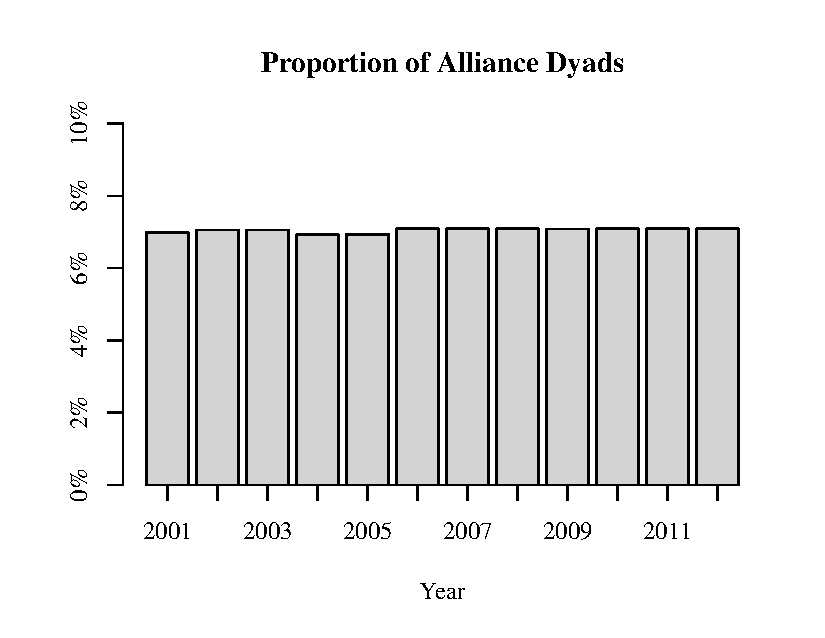
\includegraphics[height=.17\textheight, clip=true, trim=0cm 1cm 0cm 2cm]{SI_figures/descriptive_plots/alliance_barplot.pdf}    &
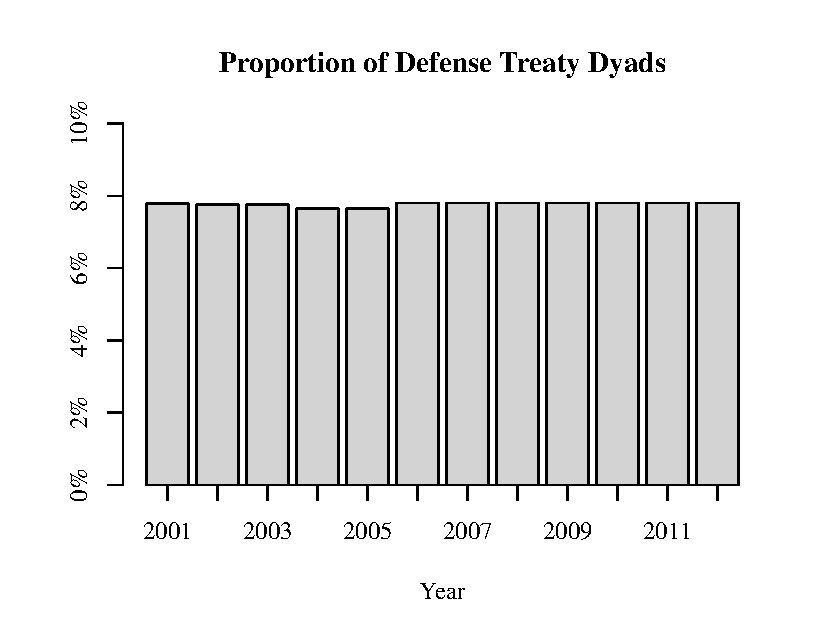
\includegraphics[height=.17\textheight, clip=true, trim=0cm 1cm 0cm 2cm]{SI_figures/descriptive_plots/defense_barplot.pdf}   \\

Bilateral Investment Treaty& OECD Pairs \\
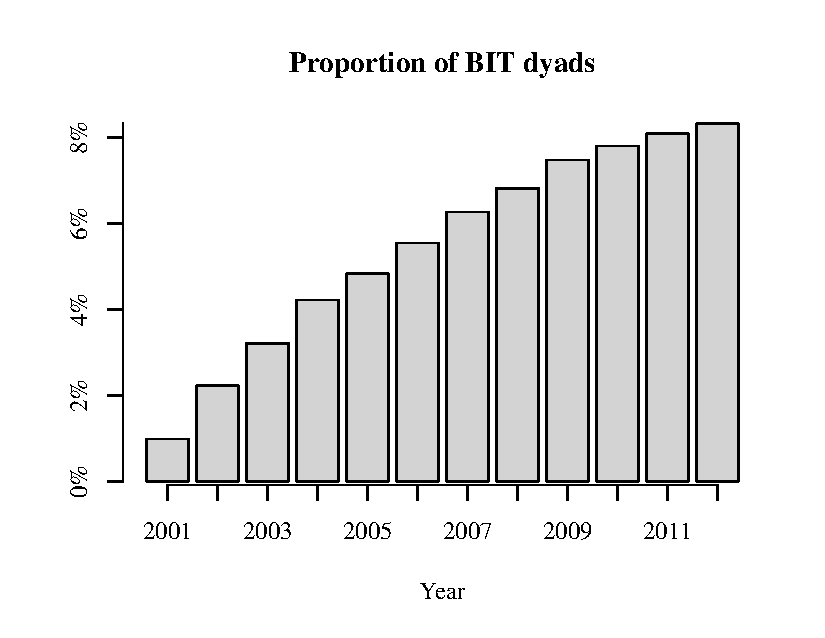
\includegraphics[height=.17\textheight, clip=true, trim=0cm 1cm 0cm 2cm]{SI_figures/descriptive_plots/BIT_barplot.pdf} &
 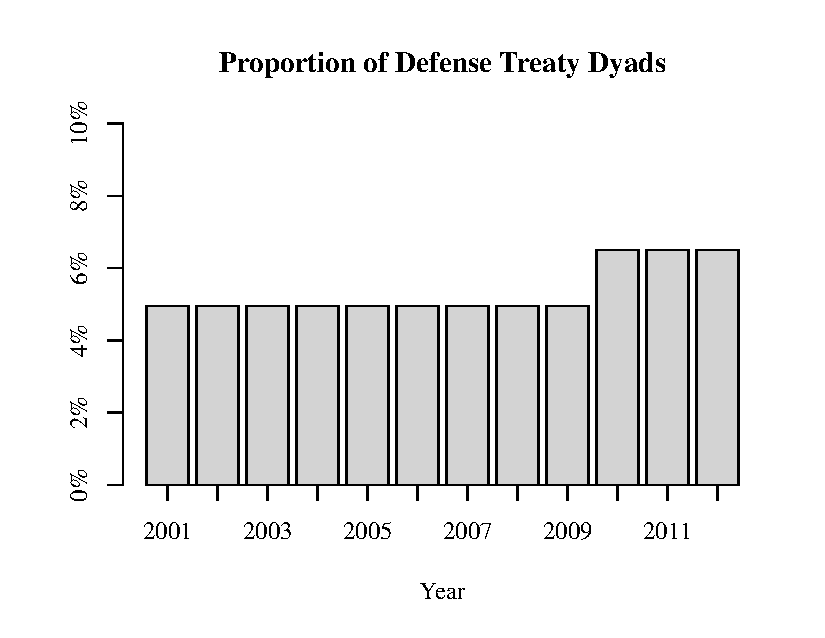
\includegraphics[height=.17\textheight, clip=true, trim=0cm 1cm 0cm 2cm]{SI_figures/descriptive_plots/OECDpair_barplot.pdf} \\

Dyad GDP Product &Distance\\
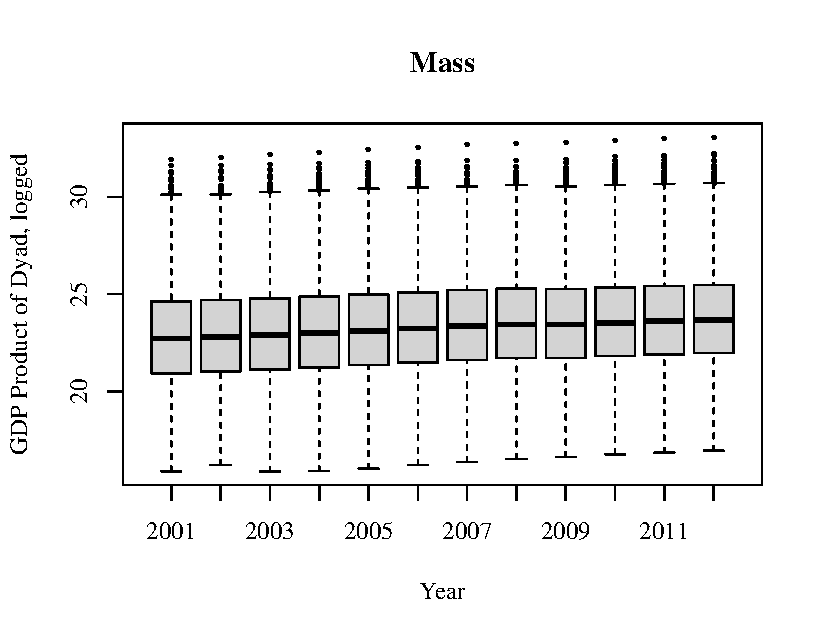
\includegraphics[height=.17\textheight, clip=true, trim=0cm 1cm 0cm 2cm]{SI_figures/descriptive_plots/Mass_boxplot.pdf}    &
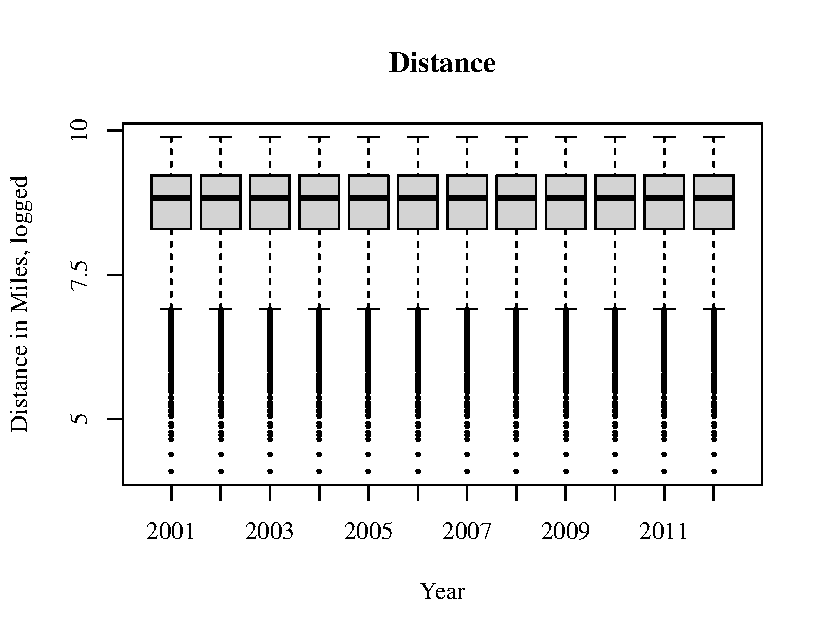
\includegraphics[height=.17\textheight, clip=true, trim=0cm 1cm 0cm 2cm]{SI_figures/descriptive_plots/dist_boxplot.pdf}   \\

GDP per capita & Polity\\
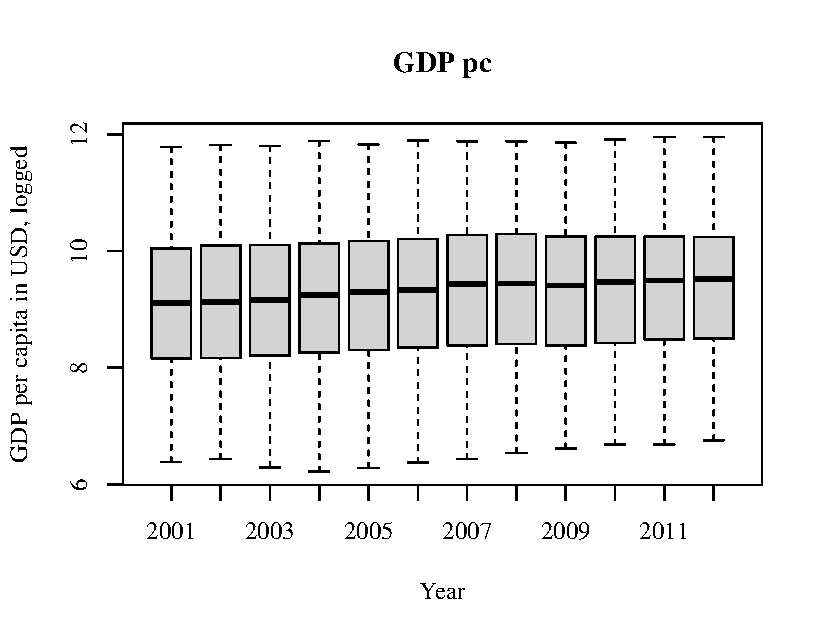
\includegraphics[height=.17\textheight, clip=true, trim=0cm 1cm 0cm 2cm]{SI_figures/descriptive_plots/GDPpc_boxplot.pdf}    &
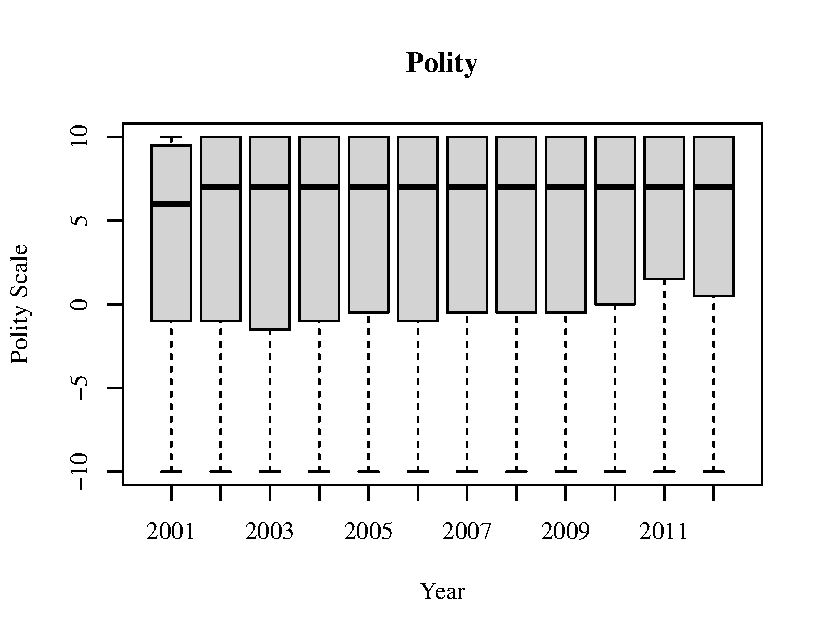
\includegraphics[height=.17\textheight, clip=true, trim=0cm 1cm 0cm 2cm]{SI_figures/descriptive_plots/polity_boxplot.pdf}  \\

\clearpage

Trade as \% of GDP &
Trade Volume\\
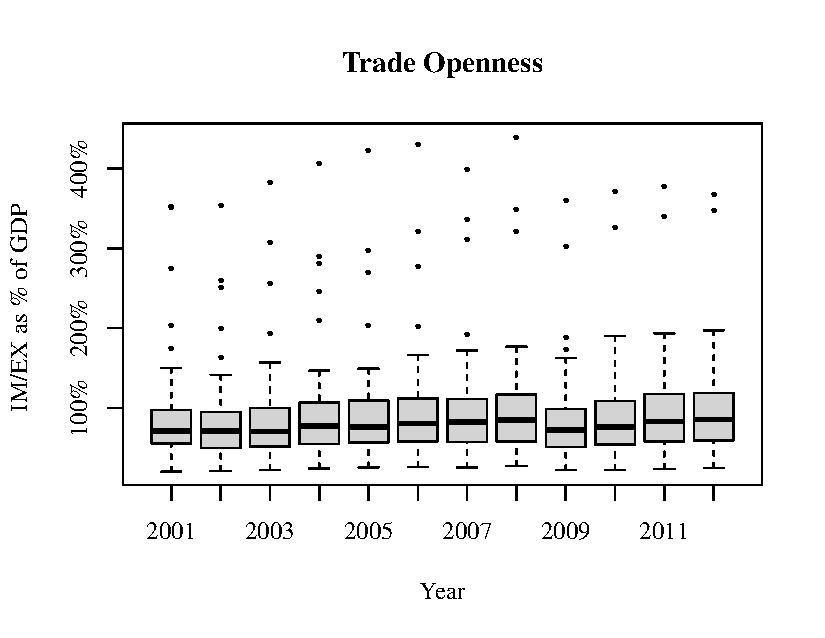
\includegraphics[height=.17\textheight, clip=true, trim=0cm 1cm 0cm 2cm]{SI_figures/descriptive_plots/TO_boxplot.pdf}   &
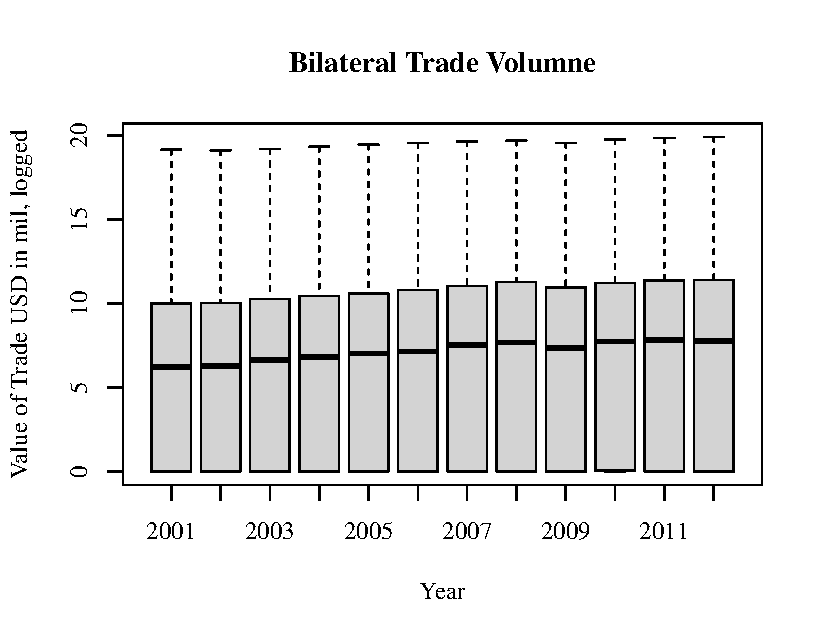
\includegraphics[height=.17\textheight, clip=true, trim=0cm 1cm 0cm 2cm]{SI_figures/descriptive_plots/Trade_boxplot.pdf}   \\

PTA Depth & FDI Stock\\
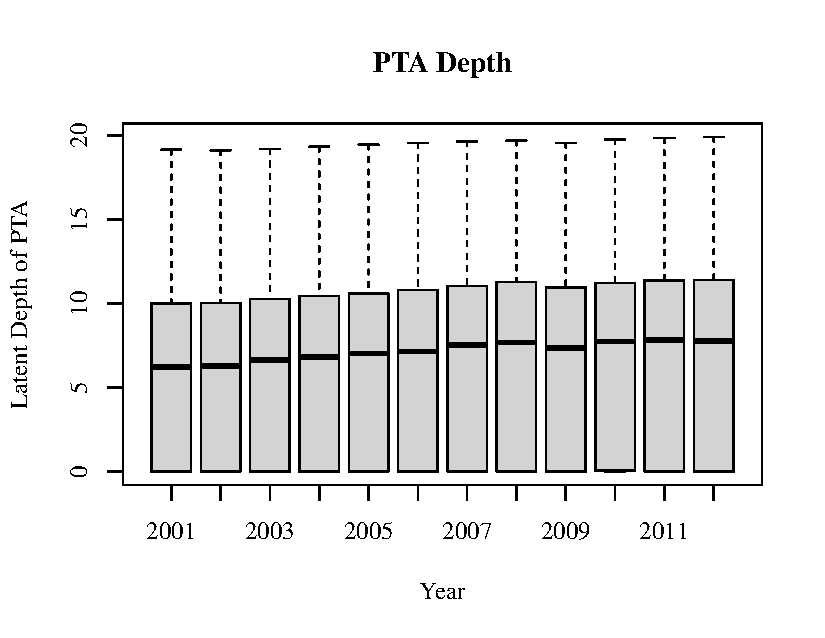
\includegraphics[height=.17\textheight, clip=true, trim=0cm 1cm 0cm 2cm]{SI_figures/descriptive_plots/ptadepth_boxplot.pdf} &
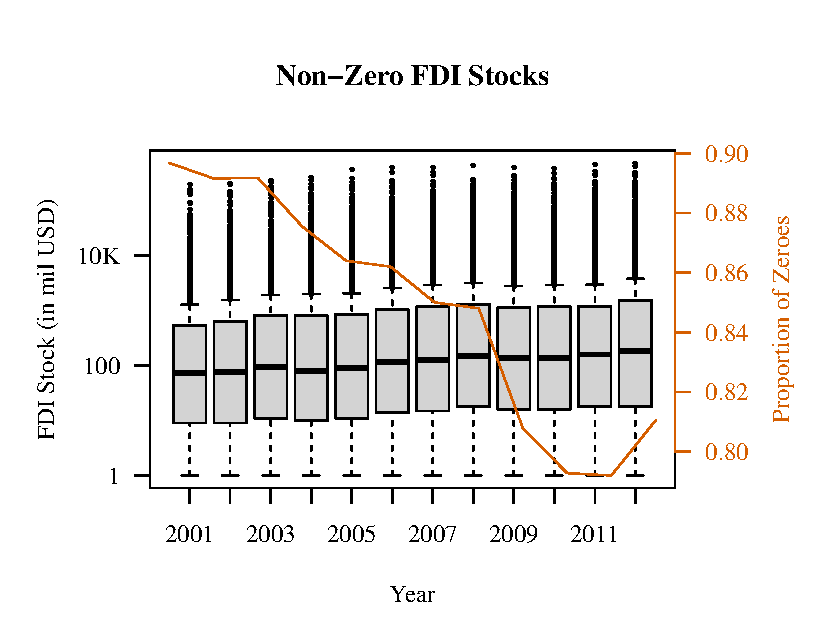
\includegraphics[height=.17\textheight, clip=true, trim=0cm 1cm 0cm 2cm]{SI_figures/descriptive_plots/fdi_stock_zeroes_boxplot.pdf}  \\


\end{longtable}




\begin{figure}[!h]
\centering
Bilateral and World FDI stocks\\
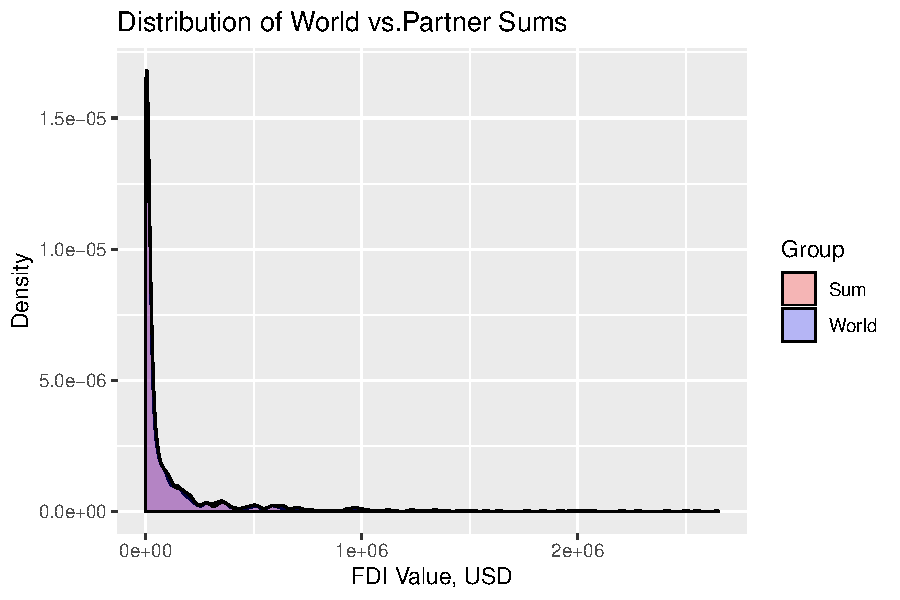
\includegraphics[height=.4\textheight, clip=true, trim=0cm 0cm 0cm .6cm]{SI_figures/descriptive_plots/check_sums.pdf} \vspace{0cm}
\caption{\label{fig:flows} Density Plot of Reported World FDI Stocks and Summed Bilateral FDI Stocks.}
\end{figure}





%\clearpage
%\begin{figure}[!h]
%\centering
%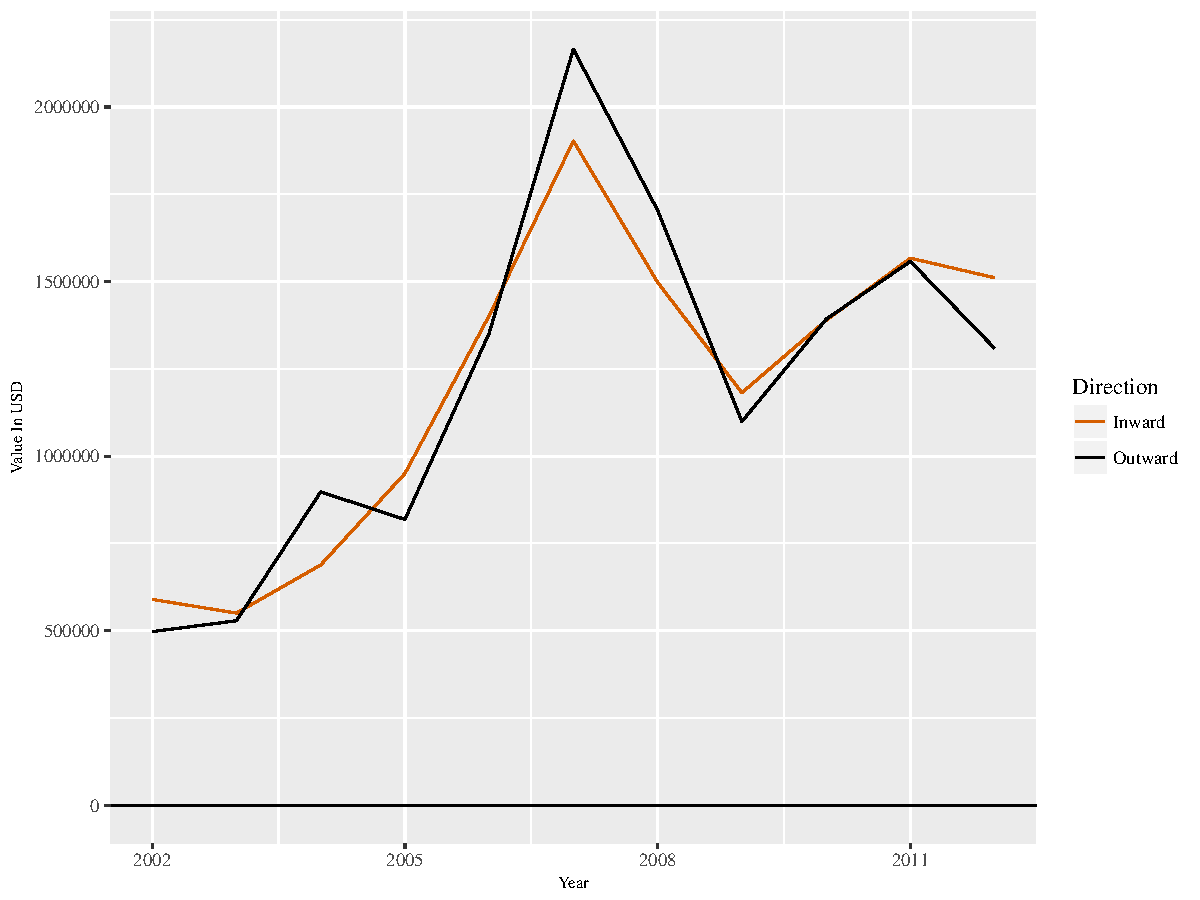
\includegraphics[height=3.5in]{SI_figures/descriptive_plots/fdi_flows.pdf} \vspace{0cm}
%\caption{\label{fig:flows} Global FDI flows by Direction.}
%\end{figure}


\section{Model and Variable Discussion}

\subsection*{Model Justification}


The steps we took to transform the dependent variable are a matter of methodological necessity.  The defining distributional feature of FDI data is zero-inflation, with there being an FDI stock of zero associated with 80--90\% of directed dyads each year. We know of two models that can currently be used to model weighted network data with zero-inflation. The first is the latent space model developed by \cite{ward2013gravity} for modeling dyadic international trade with an excess of zeros. Unfortunately, we cannot use this model to test our dependence hypotheses, since it does not permit the inclusion of structural dependence terms. The other is the count ERGM \citep{krivitsky2012exponential}, which requires dependent variable values be positive integers. A number of other models are available in the literature that could be used to evaluate dependence hypotheses and model FDI on a continuous scale if they were extended to account for zero-inflation. These include the generalized exponential random graph model (GERGM) \citep{wilson2017stochastic},  the ``AMEN'' latent factor model \citep{minhas2019inferential}, and the spatial modeling specifications proposed by \cite{neumayer2010spatial}.  We see modeling FDI stocks on the discretized logarithmic scale, as opposed to the more common continuous logarithmic scale, as an acceptable loss of information since it enables us to directly model the prevalence of zeros in the data, and to precisely test our dependence hypotheses.



\subsection*{Correlations Before and After Rounding FDI}

In this section we also investigate whether the structure of associations between FDI an the dyadic covariates included in the count ERGM is significantly changed by rounding the natural logarithm of FDI. In Table \ref{tab:cor} we present the correlation between the dyadic variables included in our ERGMs, and the pre-rounded log-FDI. In Table \ref{tab:rcor} we present the correlation between the dyadic variables and the rounded version log-FDI. In Table \ref{tab:cortest} we present two-tailed $p$-values from tests, developed by \cite{dunn1969correlation} and implemented in the \R~ package \texttt{psych} \citep{psych}, of the null hypothesis that the correlations pre and post-rounding are equal. The lowest $p$-value is 0.12, and the majority are greater than 0.50, indicating that rounding log-FDI to create a count variable does not significantly change the structure of associations in the data.

\begin{table}[!htp]
\centering
\begin{tabular}{rrrrrrrrrr}
  \hline
 & Lag FDI & GDP prod & Dist & Alliance &Defense& Trade & BIT & Both OECD & PTA \\
  \hline
2002 & 0.37 & 0.38 & -0.24 & 0.24 & 0.22 & 0.41 & 0.01 & 0.51 & 0.22 \\
  2003 & 0.39 & 0.37 & -0.25 & 0.24 & 0.22 & 0.41 & 0.01 & 0.53 & 0.24 \\
  2004 & 0.40 & 0.37 & -0.26 & 0.25 & 0.22 & 0.42 & 0.02 & 0.52 & 0.25 \\
  2005 & 0.39 & 0.40 & -0.26 & 0.26 & 0.23 & 0.44 & 0.03 & 0.50 & 0.24 \\
  2006 & 0.37 & 0.38 & -0.27 & 0.25 & 0.22 & 0.44 & 0.03 & 0.50 & 0.26 \\
  2007 & 0.36 & 0.39 & -0.28 & 0.26 & 0.23 & 0.45 & 0.04 & 0.50 & 0.31 \\
  2008 & 0.39 & 0.40 & -0.29 & 0.26 & 0.23 & 0.44 & 0.04 & 0.50 & 0.30 \\
  2009 & 0.37 & 0.43 & -0.31 & 0.28 & 0.25 & 0.48 & 0.07 & 0.49 & 0.31 \\
  2010 & 0.38 & 0.46 & -0.30 & 0.28 & 0.25 & 0.49 & 0.08 & 0.45 & 0.30 \\
  2011 & 0.39 & 0.45 & -0.30 & 0.28 & 0.25 & 0.49 & 0.08 & 0.44 & 0.30 \\
  2012 & 0.38 & 0.44 & -0.27 & 0.26 & 0.24 & 0.45 & 0.06 & 0.45 & 0.25 \\
   \hline
\end{tabular}
\caption{Correlation between dyadic variables and FDI} \label{tab:cor}
\end{table}

\begin{table}[!htp]
\centering
Correlation between dyadic variables and rounded FDI
\begin{tabular}{rrrrrrrrrr}
  \hline
 & Lag FDI & GDP prod & Dist & Alliance &Defense& Trade & BIT & Both OECD & PTA \\
  \hline
2002 & 0.36 & 0.38 & -0.24 & 0.24 & 0.21 & 0.40 & 0.01 & 0.51 & 0.22 \\
  2003 & 0.39 & 0.37 & -0.25 & 0.24 & 0.22 & 0.41 & 0.01 & 0.52 & 0.24 \\
  2004 & 0.40 & 0.37 & -0.26 & 0.25 & 0.22 & 0.42 & 0.02 & 0.52 & 0.25 \\
  2005 & 0.39 & 0.39 & -0.26 & 0.26 & 0.23 & 0.44 & 0.03 & 0.50 & 0.24 \\
  2006 & 0.36 & 0.38 & -0.27 & 0.25 & 0.22 & 0.44 & 0.03 & 0.50 & 0.26 \\
  2007 & 0.36 & 0.39 & -0.28 & 0.26 & 0.23 & 0.44 & 0.04 & 0.50 & 0.30 \\
  2008 & 0.38 & 0.40 & -0.29 & 0.25 & 0.23 & 0.44 & 0.04 & 0.50 & 0.30 \\
  2009 & 0.36 & 0.43 & -0.31 & 0.28 & 0.25 & 0.47 & 0.07 & 0.49 & 0.31 \\
  2010 & 0.37 & 0.46 & -0.30 & 0.28 & 0.25 & 0.49 & 0.08 & 0.45 & 0.30 \\
  2011 & 0.39 & 0.44 & -0.29 & 0.28 & 0.25 & 0.48 & 0.08 & 0.44 & 0.30 \\
  2012 & 0.38 & 0.44 & -0.26 & 0.26 & 0.24 & 0.45 & 0.06 & 0.44 & 0.25 \\
   \hline
\end{tabular}
\caption{Correlation between dyadic variables and FDI} \label{tab:rcor}
\end{table}


\begin{table}[!htp]
\centering
Two-tailed $p$-value in test for difference in correlations before and after rounding
\begin{tabular}{rrrrrrrrrr}
  \hline
 & Lag FDI & GDP prod & Dist & Alliance &Defense& Trade & BIT & Both OECD & PTA \\
  \hline
2002 & 0.24 & 0.57 & 0.72 & 0.65 & 0.69 & 0.58 & 1.00 & 0.47 & 0.88 \\
  2003 & 0.12 & 0.69 & 0.78 & 0.84 & 0.81 & 0.66 & 0.91 & 0.64 & 0.86 \\
  2004 & 0.22 & 0.69 & 0.66 & 0.75 & 0.72 & 0.57 & 0.91 & 0.51 & 0.75 \\
  2005 & 0.18 & 0.57 & 0.74 & 0.76 & 0.76 & 0.57 & 0.98 & 0.47 & 0.99 \\
  2006 & 0.18 & 0.68 & 0.77 & 0.76 & 0.75 & 0.65 & 0.95 & 0.43 & 0.96 \\
  2007 & 0.15 & 0.75 & 0.81 & 0.89 & 0.81 & 0.82 & 0.93 & 0.51 & 0.78 \\
  2008 & 0.19 & 0.73 & 0.71 & 0.86 & 0.89 & 0.73 & 0.98 & 0.52 & 0.84 \\
  2009 & 0.20 & 0.66 & 0.73 & 0.83 & 0.79 & 0.60 & 0.99 & 0.33 & 0.80 \\
  2010 & 0.20 & 0.71 & 0.82 & 0.90 & 0.91 & 0.68 & 1.00 & 0.52 & 0.96 \\
  2011 & 0.20 & 0.64 & 0.72 & 0.85 & 0.82 & 0.71 & 0.88 & 0.51 & 0.95 \\
  2012 & 0.23 & 0.72 & 0.73 & 0.84 & 0.88 & 0.76 & 0.87 & 0.55 & 0.92 \\
   \hline
\end{tabular}
\caption{Correlation between dyadic variables and FDI} \label{tab:cortest}
\end{table}

\subsection*{Model Fit}

To further investigate how the network model fits better than a model assumes unit independence, we compare simulated networks from the two models to the observed networks along four dimensions and for each year---a standard approach to evaluating the goodness of fit of network models \citep{hunter2008goodness}. We present quantities that evaluate the fit of the models to the reciprocity, transitivity, sender heterogeneity, and receiver heterogeneity of the networks. To measure the fit of the reciprocity, we use the weighted reciprocity measure proposed by \cite{garlaschelli2004patterns}---the correlation between the weights of edges within the same dyads. This measure ranges between -1 and 1, with higher values corresponding to a greater degree of reciprocity.  The measure we use to measure weighted transitivity comes from \cite{opsahl2009clustering}---the ratio of total transitive triple weights to total two-path weights, where the weight of a configuration is defined as the minimum value within the configuration. This measure ranges between 0 and 1, with larger values corresponding to more transitive network.  To measure receiver and sender heterogeneity, we follow \citet{minhas2019inferential} and consider the variance (presented as standard deviations) in the total received (i.e., indegree) and total sent (i.e., outdegree) by each node.

\begin{figure}[]
	\centering
	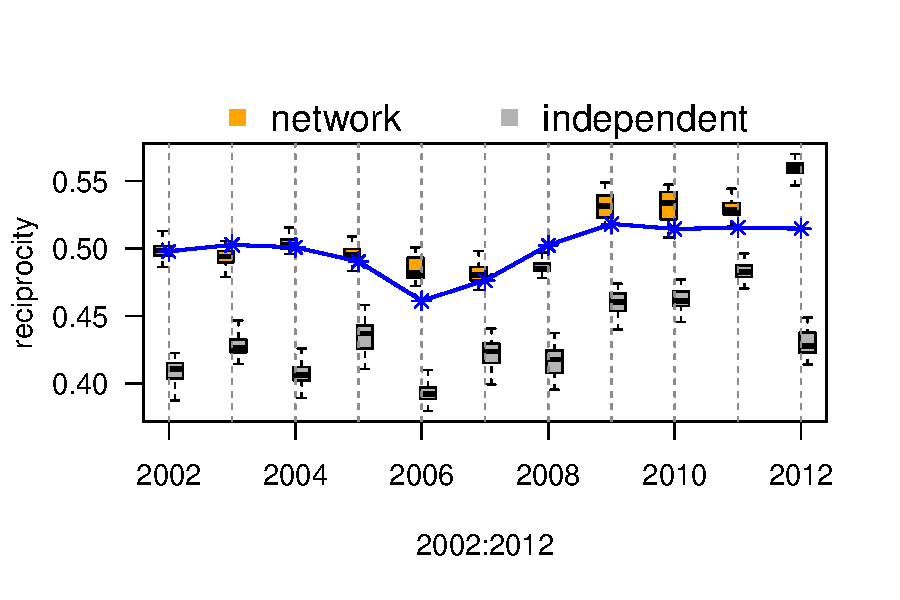
\includegraphics[scale=.75, trim = 0cm 1.5cm .1cm 0cm, clip=true  ]{figures/recip_fit.pdf}  \\
	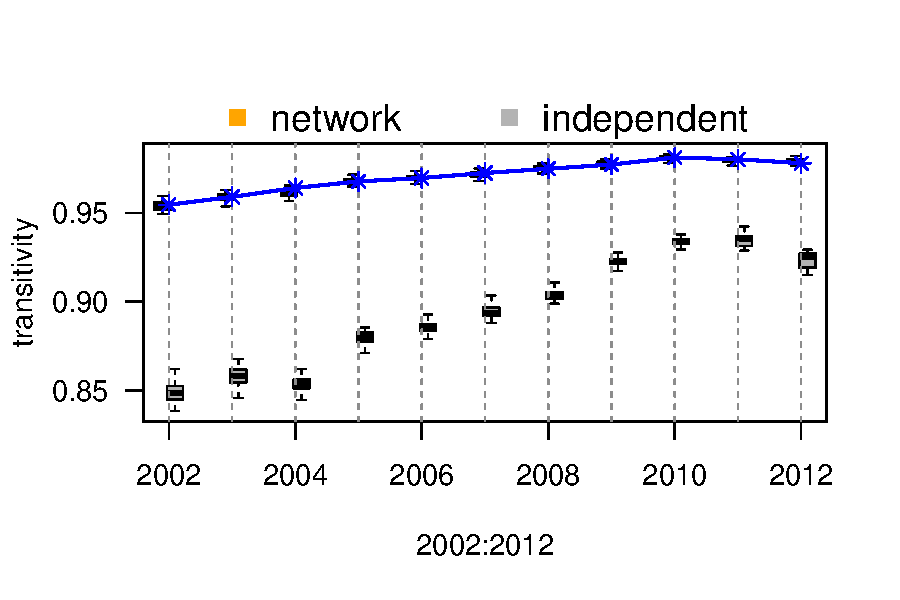
\includegraphics[scale=.75,  trim = 0cm 1.5cm .1cm 2.4cm, clip=true]{figures/trans_fit.pdf}  \\
	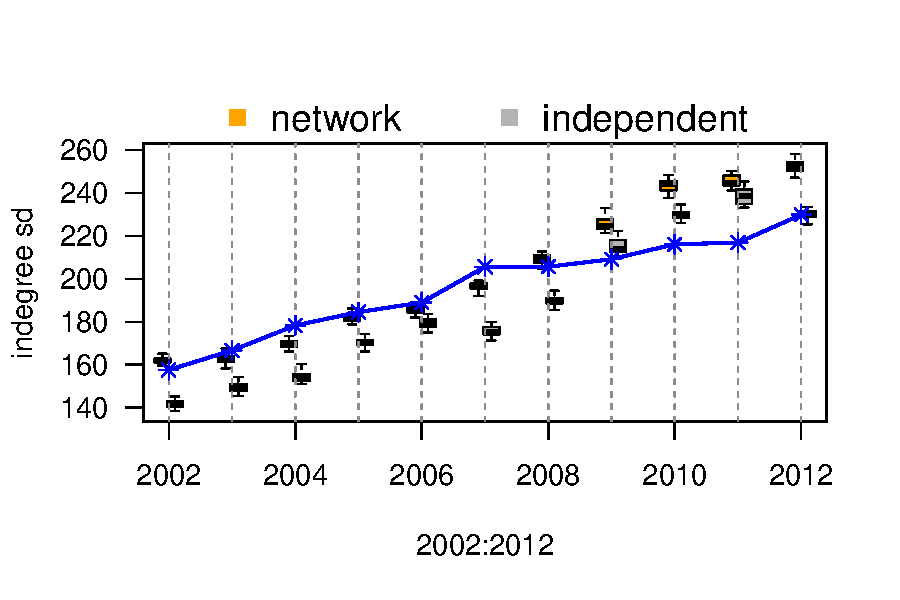
\includegraphics[scale=.75, trim = 0cm 1.5cm .1cm 2.4cm, clip=true]{figures/idsd_fit.pdf}  \\
	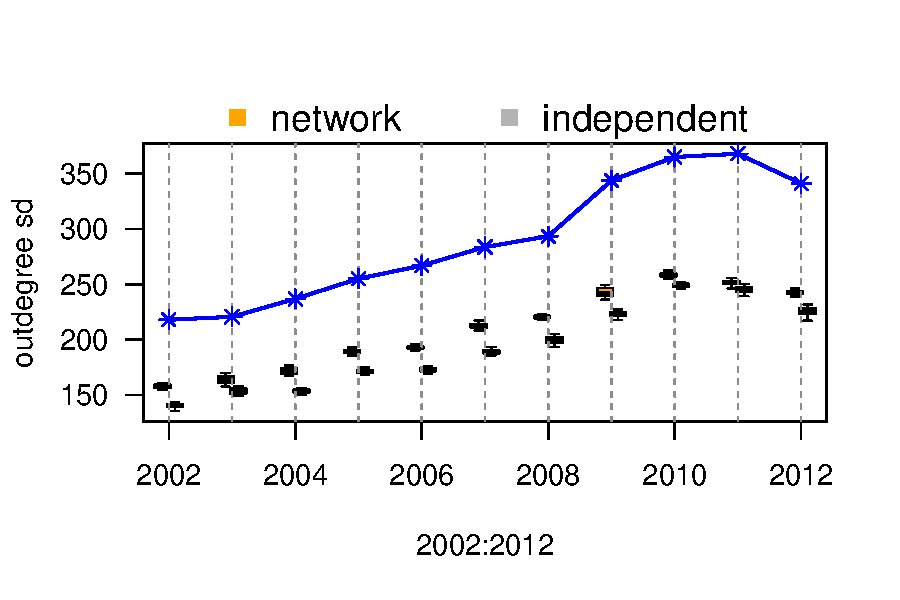
\includegraphics[scale=.75, trim = 0cm 1.5cm .1cm 2.4cm, clip=true]{figures/odsd_fit.pdf} \vspace{-.2cm}
	\caption{\label{fig:structureFit} Structural fit of the network and independence models. Boxplots depict distributions over 100 simulated networks. The orange boxplots (those to the left of the dashed vertical lines), depict distributions from the full network model. The gray boxplots depict distributions from the independence models. The blue-starred lines give the observed values. }
\end{figure}
We see in Figure \ref{fig:structureFit} that the network model provides a much better fit to the observed network than does the independent model. The boxplots depict the network statistics computed on 100 networks simulated from each model in each year. The network model fits the reciprocity and transitivity in the observed network quite well, and consistently better than does the independence model. The network model generally fits the indegree standard deviation well, but in some years the independent model provides a better fit. The one statistic that is not fit very well with either model is the outdegree standard deviation. Unfortunately, the specifications available for modeling the degree distributions in the count ERGM are still rather limited. The two statistics currently available to model degree heterogeneity---the covariance and square-root-covariance of edge values sent or received by the same node, exhibited degeneracy when fit to the FDI networks. The development of less degeneracy-prone degree statistics, such as the geometrically weighted degree terms available for binary ERGMs \citep{snijders2006new}, is an important avenue for future research with the count ERGM.

\clearpage

\section{Time-Pooled Model Results}\label{pooledresults}
For robustness checks, we re-estimate the count ERGM by pooling the data, which is common in the literature for regression based models. Figure \ref{fig:net_effects} shows that all network dependence terms are significant in the time-pooled models. Non-OECD pairs exhibit less reciprocity than OECD pairs, but the average effect for the time sample is still positive and significant.

%The exogenous covariates from the pooled model are presented in Table \ref{fig:effectPlots2}.  The results show that ignoring network structure lead to biased estimates in several covariates. We see significant differences in the coefficients for distance, the product of dyad's GDP, the three treaty variables, as well as origin and destination's GDP per capita, Polity, and trade openness. These findings are consistent with those from the yearly models. It illustrates that failure to include network structure results in biased estimates.



%\begin{landscape}
%\begin{spacing}{.7}
%\begin{longtable}[!h]{c@{\hskip .5cm}c@{\hskip .5cm}c@{\hskip .5cm}c}

%Sum & Sum$^{(1/2)}$ &Non-Zero & Alliance Treaty\\
%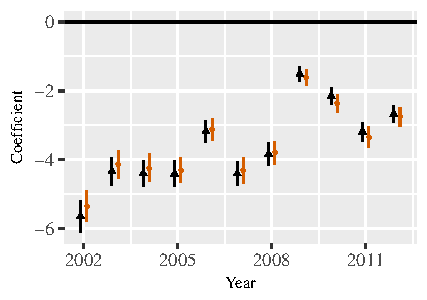
\includegraphics[height=.2\textheight, clip=true, trim=0cm 0cm 0cm .2cm]{SI_figures/plots_pooled/Sum.pdf}    &
%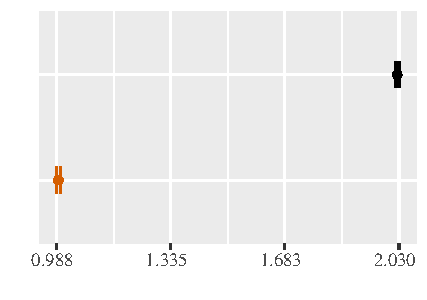
\includegraphics[height=.2\textheight, clip=true, trim=0cm 0cm 0cm .2cm]{SI_figures/plots_pooled/sum_5.pdf}   &
%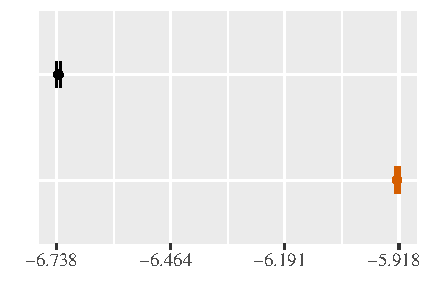
\includegraphics[height=.2\textheight, clip=true, trim=0cm 0cm 0cm .2cm]{SI_figures/plots_pooled/Non-zero.pdf} &
%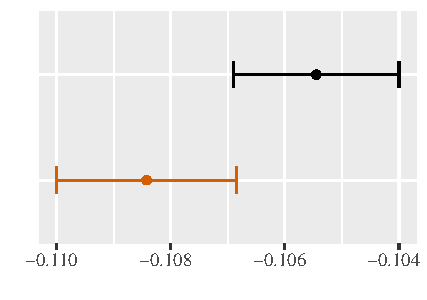
\includegraphics[height=.2\textheight, clip=true, trim=0cm 0cm 0cm .2cm]{SI_figures/plots_pooled/AllianceTreaty.pdf}   \\
%Bilateral Investment Treaty & Defense Treaty &Product of Dyad's GDP & Distance\\
%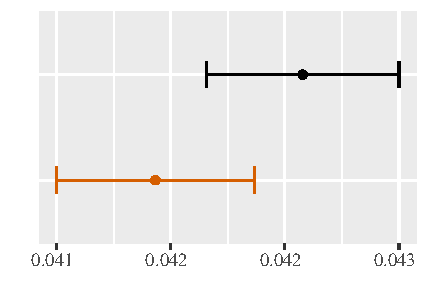
\includegraphics[height=.2\textheight, clip=true, trim=0cm 0cm 0cm .2cm]{SI_figures/plots_pooled/BIT.pdf} &
%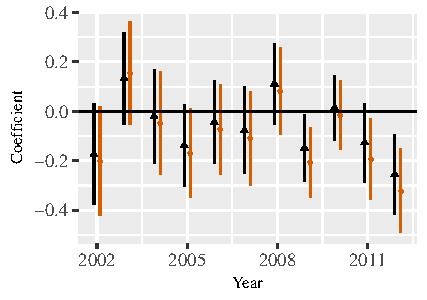
\includegraphics[height=.2\textheight, clip=true, trim=0cm 0cm 0cm .2cm]{SI_figures/plots_pooled/DefenseTreaty.pdf}   &
%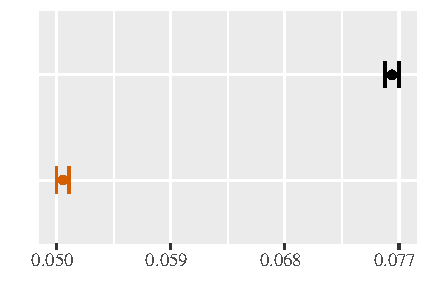
\includegraphics[height=.2\textheight, clip=true, trim=0cm 0cm 0cm .2cm]{SI_figures/plots_pooled/DyadGDPProduct.pdf} &
%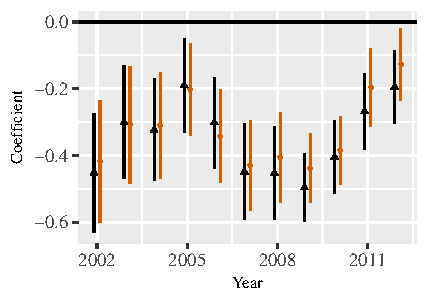
\includegraphics[height=.2\textheight, clip=true, trim=0cm 0cm 0cm .2cm]{SI_figures/plots_pooled/Distance.pdf}   \\
%Lagged FDI stock & Bilateral Trade Volume & GDP per capita, in-degree & GDP per capita, out-degree\\
%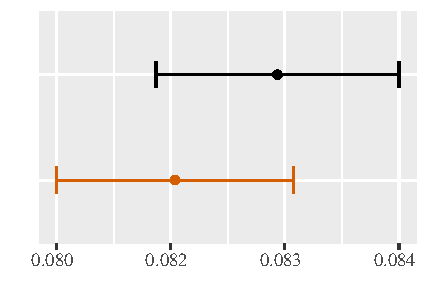
\includegraphics[height=.2\textheight, clip=true, trim=0cm 0cm 0cm .2cm]{SI_figures/plots_pooled/LaggedDV.pdf}    &
%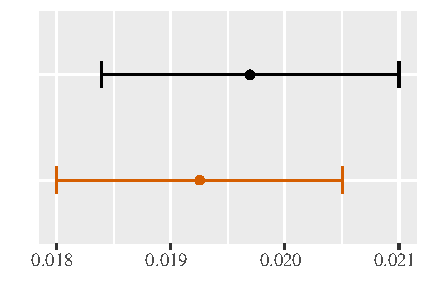
\includegraphics[height=.2\textheight, clip=true, trim=0cm 0cm 0cm .2cm]{SI_figures/plots_pooled/TradeVolume.pdf}   &
%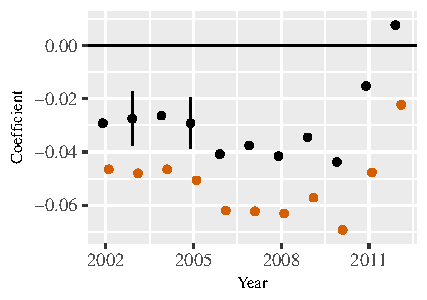
\includegraphics[height=.2\textheight, clip=true, trim=0cm 0cm 0cm .2cm]{SI_figures/plots_pooled/GDPpc_in.pdf} &
%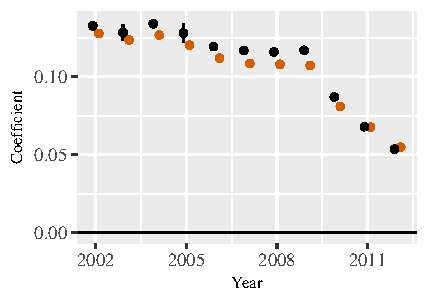
\includegraphics[height=.2\textheight, clip=true, trim=0cm 0cm 0cm .2cm]{SI_figures/plots_pooled/GDPpc_out.pdf}   \\
%Polity, in-degree & Polity, out-degree &Trade Openness, in-degree & Trade Openness, out-degree\\
%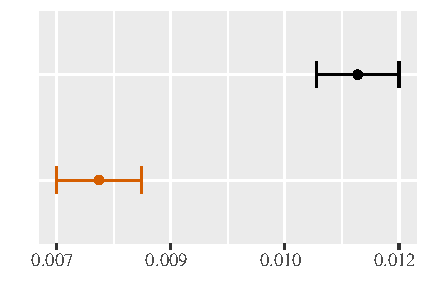
\includegraphics[height=.2\textheight, clip=true, trim=0cm 0cm 0cm .2cm]{SI_figures/plots_pooled/Polity_in.pdf} &
%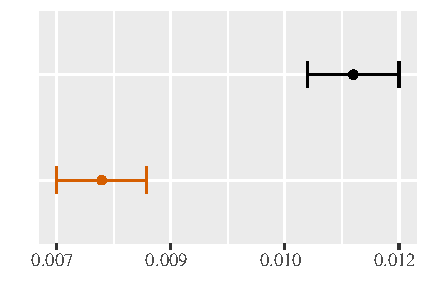
\includegraphics[height=.2\textheight, clip=true, trim=0cm 0cm 0cm .2cm]{SI_figures/plots_pooled/Polity_out.pdf}   &
%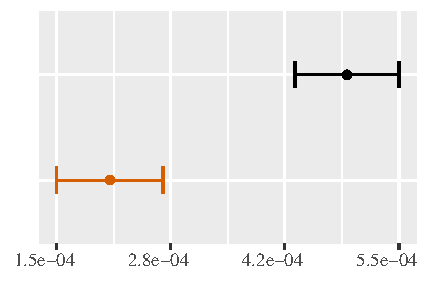
\includegraphics[height=.2\textheight, clip=true, trim=0cm 0cm 0cm .2cm]{SI_figures/plots_pooled/Trade_in.pdf} &
%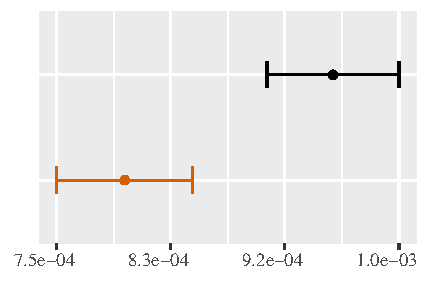
\includegraphics[height=.2\textheight, clip=true, trim=0cm 0cm 0cm .2cm]{SI_figures/plots_pooled/Trade_out.pdf}   \\

%\caption{\label{fig:effectPlots2} Estimates of terms in time-pooled ERGMs. Bars span 95\% confidence intervals. Black coefficient representations are from models excluding dependence terms (i.e., transitivity and reciprocity).}

%\end{longtable}
%\end{spacing}
%\end{landscape}


%Figure \ref{fig:exog_2}  shows that after pooling, network terms remain positive and statistically significant, supporting our hypothesis that reciprocity and transitivity characterize FDI flows. The estimates are similar to yearly results in terms of direction and statistical significance. %As expected from pooling, there are decreases in standard errors because the increased number of observations. %for variables that exhibit more yearly heterogeneity, estimates are on average more different than yearly estimates.


\begin{figure}[htp]
\centering
\begin{tabular}{@{\hskip -.05cm}c@{\hskip .2cm}c@{\hskip .2cm}c}
Transitivity  & Reciprocity, OECD pair &Reciprocity, non-OECD pair\\
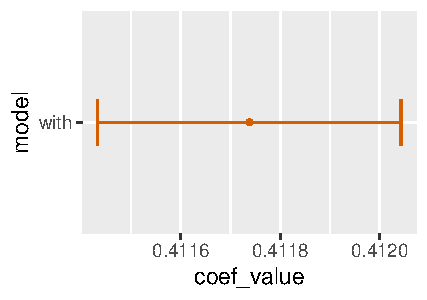
\includegraphics[height=.165\textheight, clip=true, trim=1.3cm .6cm 0cm .1cm]{SI_figures/TERGM_rl_plots/Transitivity.pdf}   &
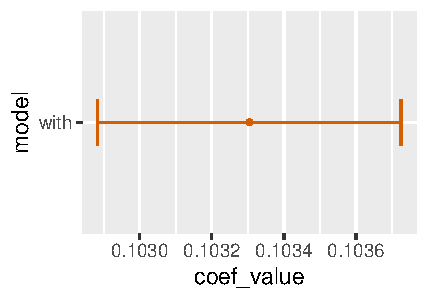
\includegraphics[height=.165\textheight, clip=true, trim=1.3cm .6cm 0cm .1cm]{SI_figures/TERGM_rl_plots/Mutuality_OECD_Pair.pdf}    &
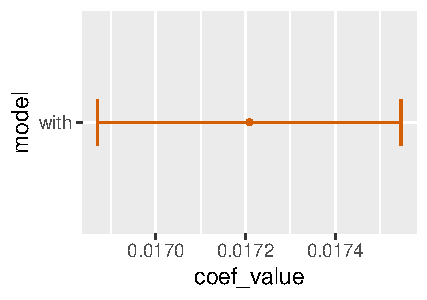
\includegraphics[height=.165\textheight, clip=true, trim=1.3cm .6cm 0cm .1cm]{SI_figures/TERGM_rl_plots/Mutuality_Not_OECD_Pair.pdf} \\
\end{tabular}
\caption{\label{fig:net_effects} Estimates of network terms in time-pooled ERGMs. Bars span 95\% confidence intervals.}
\end{figure}


\section{AME Model Results}\label{AMEresults}

As mentioned in the discussion of the GOF statistics of the main model, the count ERGM does not fit out degree actor heterogeneity very well. At the end of the day, there's no model in existence that can account for all of the peculiarities of this data (zero inflation, reciprocity, transitivity, actor heterogeneity). A relatively new latent space model called AMEN has been developed and, unlike older versions of the LSM, includes terms that can be used to account for reciprocity and transitivity \citep{minhas2019inferential}. It is also effective at accounting for actor heterogeneity, though not for zero-inflation and is not able to condition reciprocity as the ERGM does. We replicate our main model with this new model to assure that our results regarding transitivity and reciprocity are robust to accounting for actor heterogeneity. These results are estimated with the R package \texttt{amen} \citep{amen} using un-transformed FDI stock values and a Gaussian edge distribution. Below the results in Figure \ref{fig:AMEnetterms} show that both transitivity and reciprocity are significant even when better accounting for actor heterogeneity.\\


\begin{figure}[!h]
\centering
\begin{tabular}{@{\hskip -.05cm}c@{\hskip .2cm}c}
Transitivity Dependence  & Dyadic Dependence\\
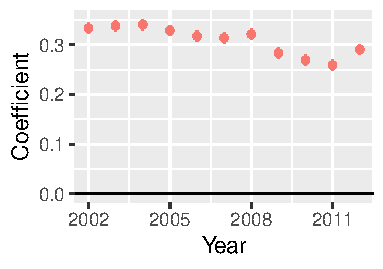
\includegraphics[height=.165\textheight, clip=true, trim=.55cm .6cm 0cm .1cm]{SI_figures/amen_rl_plots/trans.dep.pdf}   &
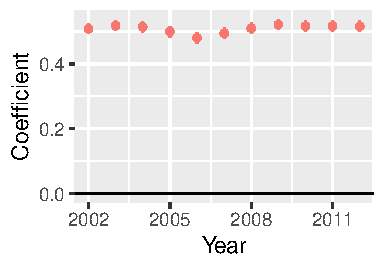
\includegraphics[height=.165\textheight, clip=true, trim=.55cm .6cm 0cm .1cm]{SI_figures/amen_rl_plots/dyad.dep.pdf} \\
\end{tabular}
\caption{\label{fig:AMEnetterms} Dependence patterns. Bars span 95\% confidence intervals. }
\end{figure}

\newpage

\section{Subset by Missingness Results}\label{qlevelresults}

The bilateral FDI data are collected mainly from national sources with technical assistance from UNCTAD; in cases where data are not available from host countries, UNCTAD uses data from partner countries (mirror data) as well as from other international organizations.\footnote{James Zhan. 2014. ``Bilateral FDI Statistics.'' \url{http://unctad.org/en/Pages/DIAE/FDI\%20Statistics/FDI-Statistics-Bilateral.aspx}, accessed April 11, 2017.} One challenge of using bilateral FDI data is the large number of unreported values. %Bilateral stock levels are self-reported and only reported if the value is not zero for all years. Because of this,
%Around 83\% of the dyadic values are missing. %This percentage would typically be considered intolerably high for statistical analysis, but one additional complication with FDI data is that
The missing values seem likely to be zero or a negligible amount (and thus not truly missing, but unreported because there was nothing to report). Comparing a country's total FDI to the sum of bilateral FDI for each year, we find that in most cases the difference is small and likely due to rounding, centering around zero (see Figure A in Appendix A). Therefore, for our main models we impute the missing values with zeros so that we have a complete data set to model network dependence.  In Appendix E, we present results using an alternative approach---subsetting to sets of countries on which we have more complete data, a common approach in dyadic research in political economy \citep[e.g., ][]{cao2014democracies,pettersson2013aid}. Our main findings regarding the effects of transitivity and reciprocity are robust to this alternative approach.  %In Appendix E, we present results using alternative approaches---multiple imputation, and subsetting to countries with more complete data. Our main findings regarding the effects of transitivity and reciprocity are robust to these alternative approaches. %To attend to the possibility that missing values are not true zeroes due to reporting biases, we use two different methods of robustness checks. The first is that we subset our data based on the amount of missingness---limiting the network to countries for which a large proportion of the bilateral data is reported. The second is that we use multiple imputations to impute the missing values and estimate the models using imputed datasets. Our main findings regarding the effects of transitivity and reciprocity remain the same when we use different approaches to address the missingness. Further discussion and the results of our robustness checks can be found in Appendix E.


In the paper, we imputed missing values with zeros. In this section, we check whether our results are robust if we analyze a subset of the data set based on the level of missingness. To subset the data, we approximate total level of missingness in the adjacency matrices ({\emph{q}) by using the proportion of missing values for each node (\emph{p}). We conduct two robustness checks: (1) when \emph{p} = 0.86,  \emph{q} $\approx$ 0.50 and  \emph{n} = 70; and (2) when \emph{p} = 0.72, \emph{q} $\approx$ 0.25 and  \emph{n} = 28. In the first case, we only include nodes with missing values that are 86\% or less of the possible edges for the entire data set, which leaves us with an adjacency matrix that is only missing 50\% of the values (70 countries in total). Similarly, the second set only includes nodes with missing values that are 72\% or less of the possible edges for the entire dataset, which leaves us with an adjacency matrix that is only missing 25\% of the values (28 countries in total).  Following our approach in the paper, we impute missing values in the two subsets of the data with zeros.

Figures \ref{fig:q50netterms} and \ref{fig:q25netterms} present the results for the two robustness checks, respectively. We see that FDI networks show strong transitivity for all years. Reciprocity effects for OECD pairs are more erratic but still significant. Reciprocity effects for non-OECD pairs follow the same pattern of starting negative and gradually becoming positive. The erratic coefficients for OECD pairs may be because the subset has substantial two-way FDI flows and thus there is little variation in the level of reciprocity.


\subsection*{q $\approx$  0.50}

\begin{figure}[!h]
\centering
\begin{tabular}{@{\hskip -.05cm}c@{\hskip .1cm}c@{\hskip .1cm}c}
Transitivity  & Reciprocity, OECD pair &Reciprocity, non-OECD pair\\
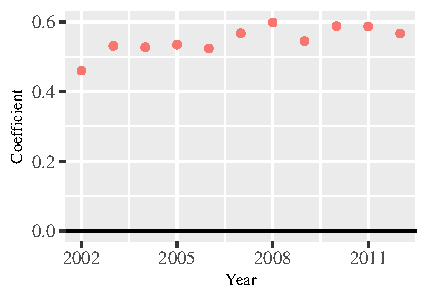
\includegraphics[height=.16\textheight, clip=true, trim=.55cm .6cm .25cm .1cm]{SI_figures/q50_rl_plots/Transitivity.pdf}   &
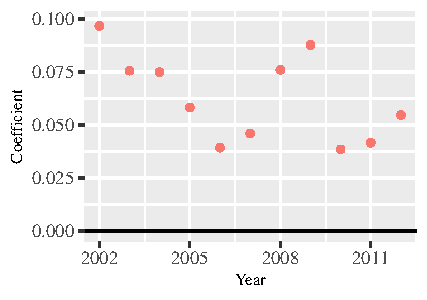
\includegraphics[height=.16\textheight, clip=true, trim=.55cm .6cm .25cm .1cm]{SI_figures/q50_rl_plots/Mutuality_OECD.pdf}    &
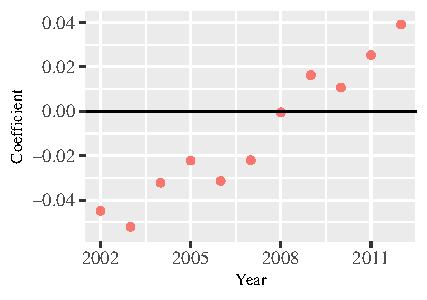
\includegraphics[height=.16\textheight, clip=true, trim=.55cm .6cm .25cm .1cm]{SI_figures/q50_rl_plots/Mutuality_notOECD.pdf} \\
\end{tabular}
\caption{\label{fig:q50netterms} Estimates of Dependence terms. Bars span 95\% confidence intervals. }
\end{figure}


\subsection*{q $\approx$  0.25}

\begin{figure}[!h]
\centering
\begin{tabular}{@{\hskip -.05cm}c@{\hskip .1cm}c@{\hskip .1cm}c}
Transitivity  & Reciprocity, OECD pair &Reciprocity, non-OECD pair\\
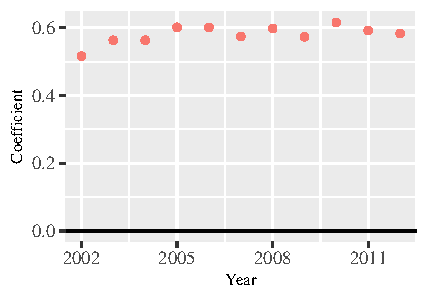
\includegraphics[height=.16\textheight, clip=true, trim=.55cm .6cm .25cm .1cm]{SI_figures/q25_rl_plots/Transitivity.pdf}   &
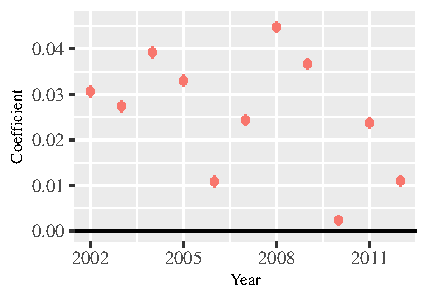
\includegraphics[height=.16\textheight, clip=true, trim=.55cm .6cm .25cm .1cm]{SI_figures/q25_rl_plots/Mutuality_OECD.pdf}    &
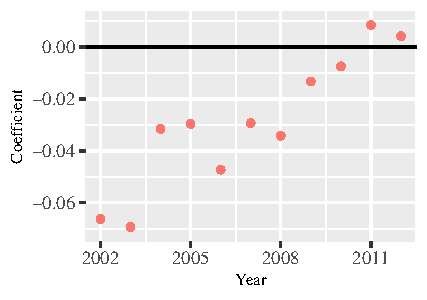
\includegraphics[height=.16\textheight, clip=true, trim=.55cm .6cm .25cm .1cm]{SI_figures/q25_rl_plots/Mutuality_notOECD.pdf} \\
\end{tabular}
\caption{\label{fig:q25netterms} Estimates of Dependence terms. Bars span 95\% confidence intervals. }
\end{figure}




%\subsection{Multiple Imputations}

%In addition to subsetting by missingness, we also employ multiple imputations using the \R{} package \texttt{Amelia}. For the imputations, we used the dataset that included all covariates and imputed the column for the original FDI stock values and then transformed the data for the models. We used ten imputations, modeled each imputed dataset and then combined the parameter estimates using standard Rubin's rules. \\

%\centerline{\textcolor{red}{WILL ADD FIGURE ONCE MODELS FINISH}}



\section{Tax Incentives and FDI}\label{taxresults}

One potential concern with bilateral FDI data is that they include round-tripping FDI, in which domestic firms transfer funds to a foreign country (typically a tax haven) and invest back as ``foreign capital'' to take advantage of preferential policies that their home countries offer to foreign investors \citep{Borga:2016}. Round-tripping FDI could inflate reciprocity. Further, firms may use tax havens to channel funds to other countries \citep{Borga:2017}. If firms in one country use a tax haven to invest in another country whose firms also invest in the former country, it creates an artificial triangle closure of investment flows (i.e., transitivity). To address these issues in bilateral FDI data and check the robustness of our findings, we re-estimated the model by including the corporate tax rate for both the sending and receiving country\footnote{Corporate tax rate data comes from the World Bank's \emph{World Development Indicators}.} and estimating models that exclude tax havens. The countries dropped as tax havens are Namibia, Trinidad and Tobago, Bahrain, Luxembourg, the United Kingdom, Ireland, and the Netherlands. We used the EU list of 17 countries as a base list, although most of them were not in our sample due to data availability.\footnote{\url{https://ec.europa.eu/taxation_customs/tax-common-eu-list_en}}  We also added Luxembourg, the United Kingdom, Ireland, and the Netherlands since they are often considered cooperative tax havens.\footnote{Matthew C. Klein. ``What the Foreign Direct Investment Data Tell Us About Corporate Tax Avoidance.'' \emph{Financial Times}, November 23, 2017. \url{https://ftalphaville.ft.com/2017/11/23/2196028/what-the-foreign-direct-investment-data-tell-us-about-corporate-tax-avoidance/}} Figure \ref{fig:tax_rates_netterms} plots the results for reciprocity and transitivity for the models with corporate tax rates. We see that the results on reciprocity become a little weaker when tax rates are included, but they remain significant in most years. Including tax rates does not affect transitivity.
Figure \ref{fig:tax_havens_netterms} plots the results for reciprocity and transitivity for the models that exclude tax havens and the results are nearly identical the main results in the paper.\\

\begin{figure}[!h]
\centering
\begin{tabular}{@{\hskip -.05cm}c@{\hskip .1cm}c@{\hskip .1cm}c}
Transitivity  & Reciprocity, OECD pair &Reciprocity, non-OECD pair\\
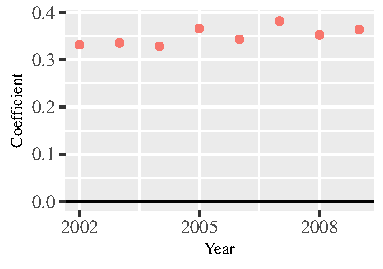
\includegraphics[height=.16\textheight, clip=true, trim=.55cm .6cm .25cm .1cm]{SI_figures/tax_rl_plots/Transitivity.pdf}   &
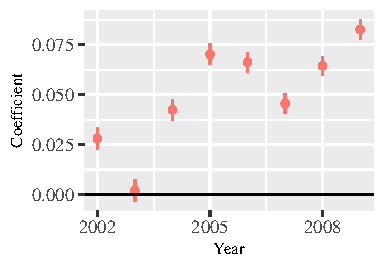
\includegraphics[height=.16\textheight, clip=true, trim=.55cm .6cm .25cm .1cm]{SI_figures/tax_rl_plots/Mutuality_OECD.pdf}    &
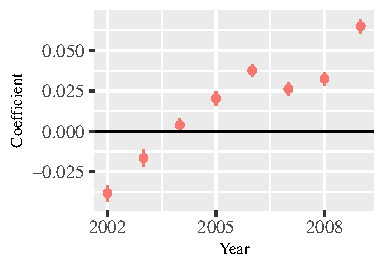
\includegraphics[height=.16\textheight, clip=true, trim=.55cm .6cm .25cm .1cm]{SI_figures/tax_rl_plots/Mutuality_notOECD.pdf} \\
\end{tabular}
\caption{\label{fig:tax_rates_netterms} Estimates of Dependence terms for models with corporate tax rates. Bars span 95\% confidence intervals. }
\end{figure}

\begin{figure}[!h]
\centering
\begin{tabular}{@{\hskip -.05cm}c@{\hskip .1cm}c@{\hskip .1cm}c}
Transitivity  & Reciprocity, OECD pair &Reciprocity, non-OECD pair\\
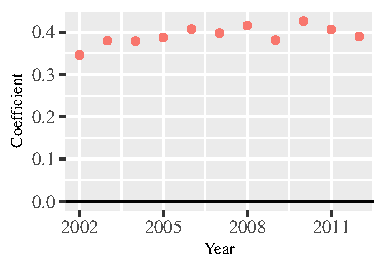
\includegraphics[height=.16\textheight, clip=true, trim=.55cm .6cm .25cm .1cm]{SI_figures/haven_rl_plots/Transitivity.pdf}   &
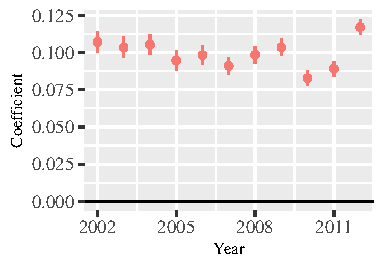
\includegraphics[height=.16\textheight, clip=true, trim=.55cm .6cm .25cm .1cm]{SI_figures/haven_rl_plots/Mutuality_OECD.pdf}    &
\includegraphics[height=.16\textheight, clip=true, trim=.55cm .6cm .25cm .1cm]{SI_figures/haven_rl_plots/Mutuality_notOECD.pdf} \\
\end{tabular}
\caption{\label{fig:tax_havens_netterms} Estimates of Dependence terms for models without tax havens. Bars span 95\% confidence intervals. }
\end{figure}


\section{Excluding the European Union}\label{EUresults}

A significant portion of the FDI in the global economy involves the European Union and the majority of the top partners for the EU are other EU countries. This is because of proximity, similar business environments and endowments, and few barriers for EU firms to send FDI to other EU countries. Because of this, there is a high degree of clustering within the EU, and so we run models that drop all EU countries to test if reciprocity and transitivity is still significant for the rest of the global economy. We find that the transitivity statistic remains largely unchanged after dropping EU countries and that reciprocity is also similar to the main results, but slightly lower and less stable. \\



\begin{figure}[!h]
\centering
\begin{tabular}{@{\hskip -.05cm}c@{\hskip .1cm}c@{\hskip .1cm}c}
Transitivity  & Reciprocity, OECD pair &Reciprocity, non-OECD pair\\
\includegraphics[height=.16\textheight, clip=true, trim=.55cm .6cm .25cm .1cm]{SI_figures/EU_rl_plots/Transitivity.pdf}   &
\includegraphics[height=.16\textheight, clip=true, trim=.55cm .6cm .25cm .1cm]{SI_figures/EU_rl_plots/Mutuality_OECD.pdf}    &
\includegraphics[height=.16\textheight, clip=true, trim=.55cm .6cm .25cm .1cm]{SI_figures/EU_rl_plots/Mutuality_notOECD.pdf} \\
\end{tabular}
\caption{\label{fig:EU_netterms} Estimates of Dependence terms. Bars span 95\% confidence intervals. }
\end{figure}

\section{Exchange rates and Inflation}\label{xrresults}

FDI stocks can vary year to year due to reasons unrelated to FDI flows, such as revaluation. While it is impossible to perfectly address this limitation of the data, we add origin and destination node level inflation and exchange rate variables to our main models to control for this. The results for transitivity remain positive and significant, but slightly lower. Reciprocity also drops for both OECD and non-OECD pairs, even becoming negative in 2007 for OECD pairs, but remains positive and significant for most years for OECD pairs and non-OECD pairs still pattern convergence by the end of the time sample.\\


\begin{figure}[!h]
\centering
\begin{tabular}{@{\hskip -.05cm}c@{\hskip .1cm}c@{\hskip .1cm}c}
Transitivity  & Reciprocity, OECD pair &Reciprocity, non-OECD pair\\
\includegraphics[height=.16\textheight, clip=true, trim=.55cm .6cm .25cm .1cm]{SI_figures/xr_rl_plots/Transitivity.pdf}   &
\includegraphics[height=.16\textheight, clip=true, trim=.55cm .6cm .25cm .1cm]{SI_figures/xr_rl_plots/Mutuality_OECD.pdf}    &
\includegraphics[height=.16\textheight, clip=true, trim=.55cm .6cm .25cm .1cm]{SI_figures/xr_rl_plots/Mutuality_notOECD.pdf} \\
\end{tabular}
\caption{\label{fig:xr_netterms} Estimates of Dependence terms. Bars span 95\% confidence intervals. }
\end{figure}


\section{Ripple Effect Simulation}\label{ripple_sim}

We investigate the interdependence in the FDI network by simulating networks after edge elimation from the full model estimated for 2012.\footnote{Our conclusions are robust to using other years---we use 2012 for consistency with the model interpretations presented in the paper.} The complete elimination of a single FDI edge would be admittedly unlikely, but the effects would be similar to that of a large reduction in an edge value, and simulating the network conditional on a fixed but non-zero edge value is much more computationally complex than eliminating an edge entirely. Another way to look at edge elimination is to consider the structural differences we would have observed if a policy was in place to prevent investment along a particular edge (e.g., via an embargo on investment).

Our objective in this simulation experiment is to understand how the elimination of an FDI edge from country $i$ to country $j$ affects the other ties to which countries $i$ and $j$ are incident. Specifically, we analyze the effects of eliminating edge $i \rightarrow j$  on four measures: (1) the expected value of FDI ties sent by $i$ to countries other than $j$, (2) the expected value of FDI ties sent by $j$, (3) the expected value of ties received by $i$, and (4) the expected value of ties received by $j$ from countries other than $i$.  These edges are ``close'' to edge $i \rightarrow j$ according to our ERGM specification in that (1) the edge sent from $j$ to $i$ factors directly into the measure of reciprocity, and (2) all edges sent to (from) $i$ and $j$ by other nodes factor into the transitive triads measure with the edge from $i$ to $j$.\footnote{Note that despite including the total amount of investment in the network (via $\text{Sum}:\bm{g(y)}$), the ERGM does not fix the sum of edges in the network---it simply generates networks with, on average, the same value of $\text{Sum}:\bm{g(y)}$ as seen in the observed network. As such, eliminating a single edge from the network will have virtually no effect on the expected values of other edges.}

There are three steps in the simulation experiment we conduct to analyze the effects of eliminating edge $i \rightarrow j$. We first simulate 500 networks from the 2012 ERGM fit. We use this sample to calculate expected values of each edge, as well as our summary measures of indirect effects, from the model without constraints on edge values (i.e., no edges eliminated). Our second step is to, for each observed edge in the 2012 networks, simulate 100 networks from the ERGM with the same parameter values, but with the respective edge value fixed to zero. Our third step is to calculate, again for each edge, the percentage change in the measures of indirect effects that result from eliminating the edge.


The results from our simulation exercise are presented in Figure \ref{fig:contagion}. We divide the edges in the network into three categories based on their expected values---small edge values (approximately 40\% of edges), between 0 and 5 on the half-log scale (i.e., \$75m USD or less); medium edge values (approximately 50\% of edges), between 5 and 15 on the half-log scale (\$75m- \$163bn USD); large edge values (approximately 10\% of edges), greater than 15 on the half-log scale (\$163bn USD and above). We see that the effects of eliminating an edge are uniformly negative for the surrounding edge---their expected values decrease.  As the expected value of the edge being eliminated increases, the magnitude of the effects on surrounding edges increases. Even for small edge values, eliminating edge $i \rightarrow j$ from the network reduces the expected values of other edges sent to/from nodes $i$ and $j$ by 2-4\%. When multiplied over dozens, or even hundreds, of ties to which two countries are incident, a 2-4\% decrease in the value of investments would represent a substantial economic shock. %If the value of edge $i \rightarrow j$ is large, the expected impact on surrounding edges grows to a 4-6\% decrease. %Our modeling highlights mechanisms through whic an economic crisis in countries at the center of the network, such as the U.S., will have a ripple effect on FDI inflows and outflows in many other countries.


\begin{figure}[!h]
\centering
\includegraphics[scale=.85]{./figures/contagion_simulation_results} \vspace{-.5cm}\\
\caption{\label{fig:contagion} Results from simulation exercise investigating the effects of eliminating edge $i \rightarrow j$. Points are drawn at the average values over all edges in the 2012 network. The bars span 95\% confidence intervals.}
\end{figure}


%\section{Contributions to the Literature}

%We make several important contributions to the literature. First, we advance the FDI literature by developing and testing a novel network theory. That is, FDI flows are determined by structures of interdependence---a class of generative processes that has been overlooked in the political economy of FDI literature that focuses heavily on domestic political institutions. %--- just as they are by conventional covariates. %We argue and empirically show that FDI flows can arise from its network interdependencies.
%FDI networks are not simply an error structure that needs to be modeled empirically, but also substantively important in explaining the pattern of cross-border investment movements. From the perspective of our network approach, a country's likelihood of receiving foreign investment depends not only on its own locational advantages such as factor endowments, market size, and institutional environments, but also on its connectivity to existing partner states in the network. %Therefore, our approach fills an important gap in the political economy of FDI literature by incorporating structures of interdependence. In the results section of this paper we include a simulation exercise using the results of our models to provide detailed interpretation of network dependence and illustrate its substantive importance. We believe this network approach has broad implications for understanding other cross-border economic exchanges such as aid, goods, services, and migrants, which are also likely to exhibit structural dependencies. %, which are central themes in the International Political Economy literature.
%Global international trade regimes, for instance, are explicitly designed based on the principle of reciprocity \citep{Bagwell_Staiger:1999}. Yet empirical studies of trade flows rarely account for the pattern of reciprocity.  %In future studies, researchers should consider using the count ERGM, or comparable models for weighted networks.

%Second, our article adds to the growing literature on the formation of global supply chains and complex production networks. The past decades have witnessed the increasing fragmentation and globalization of production, which gives rise to complex production networks that are typically coordinated by MNCs \citep{UNCTAD:2013,Baldwin:2011}. Given the intertwined linkages among firms and nations, the well-functioning of the network hinges crucially on the cooperation of each involved country. %Countries' integration into the network increases the cost of governments' opportunistic behavior that disrupts the network. %On the other hand, any shock to the network will be contagious to other countries and its adverse effects will be multiplied by the interdependence (see more discussions in Section \ref{contagion}).
%Network dependencies increase the cost of governments' opportunistic behavior and thus will likely contribute to international cooperation and peace \citep[see also][]{Dorussen_Ward:2010,Kim_Solingen:2017,johns2016under}.
%%% New post-JoP FDI paragraph %%%
%The literature on FDI has not focused on patterns of network dependence, but we argue that

%Second, understanding interdependence through FDI networks is critical to understanding the global economic system as a whole.  Recent research on interdependence in the global financial system has documented economic contagion through international trade networks \citep{kali2010financial},  international lending \citep{zakaria2017evidence,Oatley_et_al:2013}, overlapping capital ownership \citep{chuluun2017global}, and networks established through currency exchange markets \citep{matesanz2014network}. In the current paper we develop a model of the global FDI using a methodology that enables us to evaluate the ways in which an exogenous shock to one part of the network can have long-run effects on the global structure of the network (see more discussions in Section \ref{contagion}.). %For example, an economic shock to the center country of FDI networks can have a ripple effect in many other countries that are even not tied directly to the center country via FDI.

%Third, our article speaks to the ``science and the system'' debate in the International Political Economy (IPE) field \citep[see,][]{Chaudoin_Milner:2017,Oatley:2011,Chaudoin_et_al:2014,Cohen:2008,Drezner_McNamara:2013}. This debate centers on the relative importance of domestic versus systemic factors in accounting for the process of globalization. The dominant ``Open Economy Politics'' approach \citep{Lake:2009} in IPE has been criticized as the ``reductionist gamble'' because of its ignorance of system interdependence \citep{Oatley:2011}. In this article, we consider both domestic and systemic factors simultaneously and show that the pattern of FDI flows is accounted for by both domestic factors and system interdependence. Our paper joins scholars' recent efforts of bringing in systemic factors to the studies of economic globalization \cite[see,~e.g.,][]{Chaudoin_et_al:2014,ward2013gravity,cao2014democracies,Chaudoin_Wilf:2018,Hafner-Burton:2009}.

%Finally, to our knowledge, the count ERGM has not been applied previously in political science research. The count ERGM can be applied to any network in which ties are count-weighted, and therefore represents a valuable tool for political scientists, who regularly study networks with count-weighted ties (e.g., shared membership in international governmental organizations \citep{boehmke2016addressing}, the count of bills co-sponsored between legislators \citep{kirkland2013hypothesis}).%\footnote{In Appendix B we provide more discussion about why we chose the count ERGM and compare it with other model options.}




\section{Covariate interpretation}

\begin{figure}[!h]
\centering
\includegraphics[scale=.75]{./figures/tradevol_sims} \vspace{-.5cm}\\
\caption{\label{fig:tradevol} Results from the simulation exercise investigating the effects of bilateral trade volume  for year 2011. These results are from 500 simulations. The line in red is the Loess curve.}
\end{figure}

For the Poisson-reference ERGM these covariate estimates are usually interpreted by exponentiating Euler's constant to the power of the coefficient times the number of unit changes in the covariate to get the expected change in the tie weight \citep{krivitsky2013modeling}. Taking bilateral trade volume for example, if the FDI origin sent had a value of 10 logged units of trade, we would expect the value of logged FDI being sent to be 10.17 times more than if the trade volume was zero. Another method for interpreting covariate terms in the model is to simulate networks using the estimated coefficients while fixing all other covariate terms at the mean value and then comparing changes in the average edge value to the range of values of the covariate. For illustrative purpose, we present a plot of this for bilateral trade volume below in Figure \ref{fig:tradevol}. Here the plot shows that as the trade volume increases from zero to 10 logged units there is a slow increase in the average level of FDI received, but increases after 10 logged units show a much sharper increase.


\newpage
\singlespacing
\bibliographystyle{apsr}
\bibliography{fdi_reference}

\end{document}


\section{Network Visualizations}\label{visual}

Below are visualizations of the data used in our analysis. In Figure I we see that democratic regimes are more central to the network. This is also evident in Figure J, with more volume of FDI between the US and Europe than elsewhere. We use 2011 as a sample year for the visualizations.\\

\begin{figure}[!h]
\centering
\includegraphics[scale=.6, clip=true, trim=2cm 2cm 0cm 2.3cm]{SI_figures/visualizations/fdiNet2011.pdf} \vspace{0cm}
\caption{\label{fig:regime_visual} Plot for 2011. Blue to red represents a scale from more autocratic to more democratic regimes.}
\end{figure}

\begin{figure}[!h]
\centering
\includegraphics[scale=.7, clip=true, trim=0cm 9.5cm 0cm 9.5cm]{SI_figures/visualizations/fdi_map.pdf} \vspace{1cm}
\caption{\label{fig:map_visual} Map for 2011. Only includes flows for the 125 countries used in the analysis. Thicker lines represent higher values.}
\end{figure}

Table \ref{tab:describe_binary} provides means for the dichotomous dyadic variables used in our models....

% Table created by stargazer v.5.2 by Marek Hlavac, Harvard University. E-mail: hlavac at fas.harvard.edu
% Date and time: Mon, Feb 20, 2017 - 22:08:59
\begin{table}[htp] \centering
  \caption{}
  \label{}
\begin{tabular}{@{\extracolsep{5pt}}lcccc}
\\[-1.8ex]\hline
\hline \\[-1.8ex]
Statistic &  \multicolumn{1}{c}{Mean} & \multicolumn{1}{c}{St. Dev.} & \multicolumn{1}{c}{Min} & \multicolumn{1}{c}{Max} \\
\hline \\[-1.8ex]
Contiguity &  0.024 & 0.152 & 0 & 1 \\
Common Official Language &  0.112 & 0.315 & 0 & 1 \\
Common Language and Ethnicity &  0.115 & 0.318 & 0 & 1 \\
Former Colonial Relationship &  0.015 & 0.121 & 0 & 1 \\
Common Colonizer &  0.062 & 0.241 & 0 & 1 \\
Defense Treaty &  0.075 & 0.264 & 0 & 1 \\
Non-aggression Treaty &  0.064 & 0.245 & 0 & 1 \\
Neutrality Treaty &  0.004 & 0.063 & 0 & 1 \\
Entente Treaty &  0.066 & 0.248 & 0 & 1 \\
\hline \\[-1.8ex]
\end{tabular}
\caption{\label{tab:describe_binary} Descriptive statistics for dichotomous dyadic covariates. Number of observations across all years is 189,000.}
\end{table}


\includegraphics[scale=.8]{SI_figures/reciprocity.png}\\
\includegraphics[scale=.8]{SI_figures/transitivity.png}\\
\includegraphics[scale=.8]{SI_figures/assortativity.png}\\

\section{Multiple Imputations with Amelia Results}\label{ameliaresults}

%In this section, we utilize the \R{} package Amelia to impute the missing values in the full data set,  when \emph{q} $\approx$ 0.50, and when \emph{q} $\approx$ 0.25 \citep{King_et_al:2001,honaker2011amelia}. Figures \ref{fig:full_amelia_netterms} and \ref{fig:q50_amelia_netterms} show the results. We see that transitivity effects are significant in all years and reciprocity effects are also significant in most years. The results in Sections \ref{qlevelresults} and \ref{ameliaresults} give us confidence that our findings regarding the reciprocity and transitivity of FDI are not driven by the pattern of missingness in the data set.

\subsection{Full}

\begin{figure}[!h]
\centering
\begin{tabular}{c@{\hskip 0cm}c}
Reciprocity & Transitivity \\
\includegraphics[height=.2\textheight, clip=true, trim=.5cm .5cm 0cm .2cm]{SI_figures/rl_amelia_full/Mutuality.pdf}    &
\includegraphics[height=.2\textheight, clip=true, trim=.5cm .5cm 0cm .2cm]{SI_figures/rl_amelia_full/Transitivity.pdf}
\end{tabular}
\caption{\label{fig:full_amelia_netterms} Estimates of Dependence terms. Bars span 95\% confidence intervals. }
\end{figure}

\vspace*{-\baselineskip}

\subsection{q $\approx$ 0.50}

\begin{figure}[!h]
\centering
\begin{tabular}{c@{\hskip 0cm}c}
Reciprocity & Transitivity \\
\includegraphics[height=.2\textheight, clip=true, trim=.5cm .5cm 0cm .1cm]{SI_figures/rl_amelia_q50/Mutuality.pdf}    &
\includegraphics[height=.2\textheight, clip=true, trim=.5cm .5cm 0cm .1cm]{SI_figures/rl_amelia_q50/Transitivity.pdf}
\end{tabular}
\caption{\label{fig:q50_amelia_netterms} Estimates of Dependence terms. Bars span 95\% confidence intervals. }
\end{figure}

\clearpage

\subsection{q $\approx$ 0.25}

\begin{figure}[!h]
\centering
\begin{tabular}{c@{\hskip 0cm}c}
Reciprocity & Transitivity \\
\includegraphics[height=.2\textheight, clip=true, trim=.5cm .5cm 0cm .2cm]{SI_figures/rl_amelia_q25/Mutuality.pdf}    &
\includegraphics[height=.2\textheight, clip=true, trim=.5cm .5cm 0cm .2cm]{SI_figures/rl_amelia_q25/Transitivity.pdf}
\end{tabular}
\caption{\label{fig:q25_amelia_netterms} Estimates of Dependence terms. Bars span 95\% confidence intervals. }
\end{figure}

\begin{table}[!htbp] \centering
  \caption{Correlation Matrix}
  \label{}
\begin{tabular}{@{\extracolsep{5pt}} lccccccccc}
\\[-1.8ex]\hline
\hline \\[-1.8ex]
 & Mass & Distance & Polity \\
\hline \\[-1.8ex]
Mass & $1$ & $$-$0.003$ & $0.091$   \\
Distance (logged) & $$-$0.003$ & $1$ & $0.008$  \\
Polity & $0.091$ & $0.008$ & $1$  \\
Trade Openness & $$-$0.166$ & $$-$0.057$ & $$-$0.078$ \\
BITs & $0.141$ & $$-$0.085$ & $0.018$  \\
Trade Volume & $0.714$ & $$-$0.215$ & $0.215$   \\
GDP per capita (logged)& $0.392$ & $$-$0.084$ & $0.166$   \\
Alliance Treaty & $0.133$ & $$-$0.348$ & $0.073$   \\
Defense Treaty & $0.065$ & $$-$0.391$ & $0.065$ \\
\hline \\[-1.8ex]
\\[-1.8ex]\hline
\hline \\[-1.8ex]
 & Trade Openness &BITs &  Trade Volume  \\
\hline \\[-1.8ex]
Mass & $$-$0.166$ & $0.141$& $0.714$  \\
Distance (logged) & $$-$0.057$ & $$-$0.085$ & $$-$0.215$ \\
Polity & $$-$0.078$ & $0.018$& $0.215$  \\
Trade Openness  & $1$ & $0.032$ & $$-$0.055$ \\
BITs & $0.032$ & $1$ & $0.143$ \\
Trade Volume & $$-$0.055$ & $0.143$& $1$  \\
GDP per capita (logged) & $0.225$ & $0.093$ & $0.330$  \\
Alliance Treaty & $$-$0.044$ & $0.021$& $0.216$  \\
Defense Treaty & $$-$0.046$ & $0.010$ & $0.177$   \\
\hline \\[-1.8ex]
\\[-1.8ex]\hline
\hline \\[-1.8ex]
& GDP per capita & Alliance Treaty & Defense Treaty \\
\hline \\[-1.8ex]
Mass & $0.392$ & $0.133$ & $0.065$ \\
Distance & $$-$0.084$ & $$-$0.348$ & $$-$0.391$  \\
Polity & $0.166$ & $0.073$ & $0.065$   \\
Trade Openness & $0.225$ & $$-$0.044$ & $$-$0.046$\\\
BITs & $0.093$ & $0.021$ & $0.010$\\
Trade Volume & $0.330$ & $0.216$ & $0.177$ \\
GDP per capita (logged) & $1$ & $0.098$ & $0.038$ \\
Alliance Treaty & $0.098$ & $1$ & $0.850$ \\
Defense Treaty & $0.038$ & $0.850$ & $1$ \\
\hline \\[-1.8ex]
\end{tabular}
\end{table}

